\documentclass[smaller]{beamer}
\setbeameroption{hide notes}
\mode<presentation>

% font choice
% \usepackage[T1]{fontenc}
% \usepackage{kpfonts}
\usefonttheme{serif}

% Modifty the templates for title, headline and footline
\setbeamertemplate{headline}
{%
   \leavevmode%
   \hbox{\begin{beamercolorbox}[wd=.75\paperwidth,ht=2.5ex,dp=1.125ex,leftskip=.3cm,rightskip=.3cm plus1fill]{author in head/foot}%
     \usebeamerfont{author in head/foot}Learned transform compression with optimized entropy encoding
   \end{beamercolorbox}%
   \begin{beamercolorbox}[wd=.25\paperwidth,ht=2.5ex,dp=1.125ex,leftskip=.3cm,rightskip=.3cm plus1fil]{title in head/foot}%
     \usebeamerfont{title in head/foot}\insertsection %\insertshorttitle
   \end{beamercolorbox}}%
   \vskip0pt%
}

\setbeamertemplate{footline}
{
  \leavevmode%
  \hbox{%
  \begin{beamercolorbox}[wd=.5\paperwidth,ht=2.25ex,dp=1ex,leftskip=0.3cm]{author in head/foot}%
    \usebeamerfont{date in head/foot}Magda Gregorov\'a, 26/3/2021, W\"urzburg, Germany
  \end{beamercolorbox}%
  \begin{beamercolorbox}[wd=.5\paperwidth,ht=2.25ex,dp=1ex,rightskip=0.3cm]{title in head/foot}%
    \usebeamerfont{title in head/foot}\hfill \insertframenumber{} / \inserttotalframenumber 
  \end{beamercolorbox}%
  }%
  \vskip0pt%
}
\makeatother

% smaller font for tables
\def\tablesize{\@setsize\tablesize{5pt}\viipt\@viipt} 

% absolute positioning
\usepackage[absolute,overlay]{textpos}

% for transparent text
% \newcommand{\semitransp}[2][35]{\color{fg!#1}#2}
% \setbeamercovered{transparent}
% \setbeamercovered{
%     still covered={\opaqueness<1->{5}},
%     again covered={\opaqueness<1->{5}}
% }

% path to images
\graphicspath{{Pics/}}

% bibliography
\bibliographystyle{alpha}

\newif\ifcuboidshade
\newif\ifcuboidemphedge

%% ========== tikz pictures ========== %%
\usepackage{tikz}

% From here: https://tex.stackexchange.com/questions/29877/need-help-creating-a-3d-cube-from-a-2d-set-of-nodes-in-tikz/387530

\tikzset{
  cuboid/.is family,
  cuboid,
  shiftx/.initial=0,
  shifty/.initial=0,
  dimx/.initial=3,
  dimy/.initial=3,
  dimz/.initial=3,
  scale/.initial=1,
  densityx/.initial=1,
  densityy/.initial=1,
  densityz/.initial=1,
  rotation/.initial=0,
  anglex/.initial=0,
  angley/.initial=90,
  anglez/.initial=225,
  scalex/.initial=1,
  scaley/.initial=1,
  scalez/.initial=0.5,
  front/.style={draw=black,fill=white},
  top/.style={draw=black,fill=white},
  right/.style={draw=black,fill=white},
  shade/.is if=cuboidshade,
  shadecolordark/.initial=black,
  shadecolorlight/.initial=white,
  shadeopacity/.initial=0.15,
  shadesamples/.initial=16,
  emphedge/.is if=cuboidemphedge,
  emphstyle/.style={thick},
}

\newcommand{\tikzcuboidkey}[1]{\pgfkeysvalueof{/tikz/cuboid/#1}}

% Commands
\newcommand{\tikzcuboid}[1]{
    \tikzset{cuboid,#1} % Process Keys passed to command
  \pgfmathsetlengthmacro{\vectorxx}{\tikzcuboidkey{scalex}*cos(\tikzcuboidkey{anglex})*28.452756}
  \pgfmathsetlengthmacro{\vectorxy}{\tikzcuboidkey{scalex}*sin(\tikzcuboidkey{anglex})*28.452756}
  \pgfmathsetlengthmacro{\vectoryx}{\tikzcuboidkey{scaley}*cos(\tikzcuboidkey{angley})*28.452756}
  \pgfmathsetlengthmacro{\vectoryy}{\tikzcuboidkey{scaley}*sin(\tikzcuboidkey{angley})*28.452756}
  \pgfmathsetlengthmacro{\vectorzx}{\tikzcuboidkey{scalez}*cos(\tikzcuboidkey{anglez})*28.452756}
  \pgfmathsetlengthmacro{\vectorzy}{\tikzcuboidkey{scalez}*sin(\tikzcuboidkey{anglez})*28.452756}
  \begin{scope}[xshift=\tikzcuboidkey{shiftx}, yshift=\tikzcuboidkey{shifty}, scale=\tikzcuboidkey{scale}, rotate=\tikzcuboidkey{rotation}, x={(\vectorxx,\vectorxy)}, y={(\vectoryx,\vectoryy)}, z={(\vectorzx,\vectorzy)}]
    \pgfmathsetmacro{\steppingx}{1/\tikzcuboidkey{densityx}}
  \pgfmathsetmacro{\steppingy}{1/\tikzcuboidkey{densityy}}
  \pgfmathsetmacro{\steppingz}{1/\tikzcuboidkey{densityz}}
  \newcommand{\dimx}{\tikzcuboidkey{dimx}}
  \newcommand{\dimy}{\tikzcuboidkey{dimy}}
  \newcommand{\dimz}{\tikzcuboidkey{dimz}}
  \pgfmathsetmacro{\secondx}{2*\steppingx}
  \pgfmathsetmacro{\secondy}{2*\steppingy}
  \pgfmathsetmacro{\secondz}{2*\steppingz}
  \foreach \x in {\steppingx,\secondx,...,\dimx}
  { \foreach \y in {\steppingy,\secondy,...,\dimy}
    {   \pgfmathsetmacro{\lowx}{(\x-\steppingx)}
      \pgfmathsetmacro{\lowy}{(\y-\steppingy)}
      \filldraw[cuboid/front] (\lowx,\lowy,\dimz) -- (\lowx,\y,\dimz) -- (\x,\y,\dimz) -- (\x,\lowy,\dimz) -- cycle;
    }
    }
  \foreach \x in {\steppingx,\secondx,...,\dimx}
  { \foreach \z in {\steppingz,\secondz,...,\dimz}
    {   \pgfmathsetmacro{\lowx}{(\x-\steppingx)}
      \pgfmathsetmacro{\lowz}{(\z-\steppingz)}
      \filldraw[cuboid/top] (\lowx,\dimy,\lowz) -- (\lowx,\dimy,\z) -- (\x,\dimy,\z) -- (\x,\dimy,\lowz) -- cycle;
        }
    }
    \foreach \y in {\steppingy,\secondy,...,\dimy}
  { \foreach \z in {\steppingz,\secondz,...,\dimz}
    {   \pgfmathsetmacro{\lowy}{(\y-\steppingy)}
      \pgfmathsetmacro{\lowz}{(\z-\steppingz)}
      \filldraw[cuboid/right] (\dimx,\lowy,\lowz) -- (\dimx,\lowy,\z) -- (\dimx,\y,\z) -- (\dimx,\y,\lowz) -- cycle;
    }
  }
  \ifcuboidemphedge
    \draw[cuboid/emphstyle] (0,\dimy,0) -- (\dimx,\dimy,0) -- (\dimx,\dimy,\dimz) -- (0,\dimy,\dimz) -- cycle;%
    \draw[cuboid/emphstyle] (0,\dimy,\dimz) -- (0,0,\dimz) -- (\dimx,0,\dimz) -- (\dimx,\dimy,\dimz);%
    \draw[cuboid/emphstyle] (\dimx,\dimy,0) -- (\dimx,0,0) -- (\dimx,0,\dimz);%
    \fi

    \ifcuboidshade
    \pgfmathsetmacro{\cstepx}{\dimx/\tikzcuboidkey{shadesamples}}
    \pgfmathsetmacro{\cstepy}{\dimy/\tikzcuboidkey{shadesamples}}
    \pgfmathsetmacro{\cstepz}{\dimz/\tikzcuboidkey{shadesamples}}
    \foreach \s in {1,...,\tikzcuboidkey{shadesamples}}
    {   \pgfmathsetmacro{\lows}{\s-1}
        \pgfmathsetmacro{\cpercent}{(\lows)/(\tikzcuboidkey{shadesamples}-1)*100}
        \fill[opacity=\tikzcuboidkey{shadeopacity},color=\tikzcuboidkey{shadecolorlight}!\cpercent!\tikzcuboidkey{shadecolordark}] (0,\s*\cstepy,\dimz) -- (\s*\cstepx,\s*\cstepy,\dimz) -- (\s*\cstepx,0,\dimz) -- (\lows*\cstepx,0,\dimz) -- (\lows*\cstepx,\lows*\cstepy,\dimz) -- (0,\lows*\cstepy,\dimz) -- cycle;
        \fill[opacity=\tikzcuboidkey{shadeopacity},color=\tikzcuboidkey{shadecolorlight}!\cpercent!\tikzcuboidkey{shadecolordark}] (0,\dimy,\s*\cstepz) -- (\s*\cstepx,\dimy,\s*\cstepz) -- (\s*\cstepx,\dimy,0) -- (\lows*\cstepx,\dimy,0) -- (\lows*\cstepx,\dimy,\lows*\cstepz) -- (0,\dimy,\lows*\cstepz) -- cycle;
        \fill[opacity=\tikzcuboidkey{shadeopacity},color=\tikzcuboidkey{shadecolorlight}!\cpercent!\tikzcuboidkey{shadecolordark}] (\dimx,0,\s*\cstepz) -- (\dimx,\s*\cstepy,\s*\cstepz) -- (\dimx,\s*\cstepy,0) -- (\dimx,\lows*\cstepy,0) -- (\dimx,\lows*\cstepy,\lows*\cstepz) -- (\dimx,0,\lows*\cstepz) -- cycle;
    }
    \fi 

  \end{scope}
}

% Optional math commands from https://github.com/goodfeli/dlbook_notation.
%%%%% NEW MATH DEFINITIONS %%%%%

\usepackage{amsmath,amsfonts,bm}

% Mark sections of captions for referring to divisions of figures
\newcommand{\figleft}{{\em (Left)}}
\newcommand{\figcenter}{{\em (Center)}}
\newcommand{\figright}{{\em (Right)}}
\newcommand{\figtop}{{\em (Top)}}
\newcommand{\figbottom}{{\em (Bottom)}}
\newcommand{\captiona}{{\em (a)}}
\newcommand{\captionb}{{\em (b)}}
\newcommand{\captionc}{{\em (c)}}
\newcommand{\captiond}{{\em (d)}}

% Highlight a newly defined term
\newcommand{\newterm}[1]{{\bf #1}}


% Figure reference, lower-case.
\def\figref#1{figure~\ref{#1}}
% Figure reference, capital. For start of sentence
\def\Figref#1{Figure~\ref{#1}}
\def\twofigref#1#2{figures \ref{#1} and \ref{#2}}
\def\quadfigref#1#2#3#4{figures \ref{#1}, \ref{#2}, \ref{#3} and \ref{#4}}
% Section reference, lower-case.
\def\secref#1{section~\ref{#1}}
% Section reference, capital.
\def\Secref#1{Section~\ref{#1}}
% Reference to two sections.
\def\twosecrefs#1#2{sections \ref{#1} and \ref{#2}}
% Reference to three sections.
\def\secrefs#1#2#3{sections \ref{#1}, \ref{#2} and \ref{#3}}
% Reference to an equation, lower-case.
\def\eqref#1{equation~\ref{#1}}
% Reference to an equation, upper case
\def\Eqref#1{Equation~\ref{#1}}
% A raw reference to an equation---avoid using if possible
\def\plaineqref#1{\ref{#1}}
% Reference to a chapter, lower-case.
\def\chapref#1{chapter~\ref{#1}}
% Reference to an equation, upper case.
\def\Chapref#1{Chapter~\ref{#1}}
% Reference to a range of chapters
\def\rangechapref#1#2{chapters\ref{#1}--\ref{#2}}
% Reference to an algorithm, lower-case.
\def\algref#1{algorithm~\ref{#1}}
% Reference to an algorithm, upper case.
\def\Algref#1{Algorithm~\ref{#1}}
\def\twoalgref#1#2{algorithms \ref{#1} and \ref{#2}}
\def\Twoalgref#1#2{Algorithms \ref{#1} and \ref{#2}}
% Reference to a part, lower case
\def\partref#1{part~\ref{#1}}
% Reference to a part, upper case
\def\Partref#1{Part~\ref{#1}}
\def\twopartref#1#2{parts \ref{#1} and \ref{#2}}

\def\ceil#1{\lceil #1 \rceil}
\def\floor#1{\lfloor #1 \rfloor}
\def\1{\bm{1}}
\newcommand{\train}{\mathcal{D}}
\newcommand{\valid}{\mathcal{D_{\mathrm{valid}}}}
\newcommand{\test}{\mathcal{D_{\mathrm{test}}}}

\def\eps{{\epsilon}}


% Random variables
\def\reta{{\textnormal{$\eta$}}}
\def\ra{{\textnormal{a}}}
\def\rb{{\textnormal{b}}}
\def\rc{{\textnormal{c}}}
\def\rd{{\textnormal{d}}}
\def\re{{\textnormal{e}}}
\def\rf{{\textnormal{f}}}
\def\rg{{\textnormal{g}}}
\def\rh{{\textnormal{h}}}
\def\ri{{\textnormal{i}}}
\def\rj{{\textnormal{j}}}
\def\rk{{\textnormal{k}}}
\def\rl{{\textnormal{l}}}
% rm is already a command, just don't name any random variables m
\def\rn{{\textnormal{n}}}
\def\ro{{\textnormal{o}}}
\def\rp{{\textnormal{p}}}
\def\rq{{\textnormal{q}}}
\def\rr{{\textnormal{r}}}
\def\rs{{\textnormal{s}}}
\def\rt{{\textnormal{t}}}
\def\ru{{\textnormal{u}}}
\def\rv{{\textnormal{v}}}
\def\rw{{\textnormal{w}}}
\def\rx{{\textnormal{x}}}
\def\ry{{\textnormal{y}}}
\def\rz{{\textnormal{z}}}

% Random vectors
\def\rvepsilon{{\mathbf{\epsilon}}}
\def\rvtheta{{\mathbf{\theta}}}
\def\rva{{\mathbf{a}}}
\def\rvb{{\mathbf{b}}}
\def\rvc{{\mathbf{c}}}
\def\rvd{{\mathbf{d}}}
\def\rve{{\mathbf{e}}}
\def\rvf{{\mathbf{f}}}
\def\rvg{{\mathbf{g}}}
\def\rvh{{\mathbf{h}}}
\def\rvu{{\mathbf{i}}}
\def\rvj{{\mathbf{j}}}
\def\rvk{{\mathbf{k}}}
\def\rvl{{\mathbf{l}}}
\def\rvm{{\mathbf{m}}}
\def\rvn{{\mathbf{n}}}
\def\rvo{{\mathbf{o}}}
\def\rvp{{\mathbf{p}}}
\def\rvq{{\mathbf{q}}}
\def\rvr{{\mathbf{r}}}
\def\rvs{{\mathbf{s}}}
\def\rvt{{\mathbf{t}}}
\def\rvu{{\mathbf{u}}}
\def\rvv{{\mathbf{v}}}
\def\rvw{{\mathbf{w}}}
\def\rvx{{\mathbf{x}}}
\def\rvy{{\mathbf{y}}}
\def\rvz{{\mathbf{z}}}

% Elements of random vectors
\def\erva{{\textnormal{a}}}
\def\ervb{{\textnormal{b}}}
\def\ervc{{\textnormal{c}}}
\def\ervd{{\textnormal{d}}}
\def\erve{{\textnormal{e}}}
\def\ervf{{\textnormal{f}}}
\def\ervg{{\textnormal{g}}}
\def\ervh{{\textnormal{h}}}
\def\ervi{{\textnormal{i}}}
\def\ervj{{\textnormal{j}}}
\def\ervk{{\textnormal{k}}}
\def\ervl{{\textnormal{l}}}
\def\ervm{{\textnormal{m}}}
\def\ervn{{\textnormal{n}}}
\def\ervo{{\textnormal{o}}}
\def\ervp{{\textnormal{p}}}
\def\ervq{{\textnormal{q}}}
\def\ervr{{\textnormal{r}}}
\def\ervs{{\textnormal{s}}}
\def\ervt{{\textnormal{t}}}
\def\ervu{{\textnormal{u}}}
\def\ervv{{\textnormal{v}}}
\def\ervw{{\textnormal{w}}}
\def\ervx{{\textnormal{x}}}
\def\ervy{{\textnormal{y}}}
\def\ervz{{\textnormal{z}}}

% Random matrices
\def\rmA{{\mathbf{A}}}
\def\rmB{{\mathbf{B}}}
\def\rmC{{\mathbf{C}}}
\def\rmD{{\mathbf{D}}}
\def\rmE{{\mathbf{E}}}
\def\rmF{{\mathbf{F}}}
\def\rmG{{\mathbf{G}}}
\def\rmH{{\mathbf{H}}}
\def\rmI{{\mathbf{I}}}
\def\rmJ{{\mathbf{J}}}
\def\rmK{{\mathbf{K}}}
\def\rmL{{\mathbf{L}}}
\def\rmM{{\mathbf{M}}}
\def\rmN{{\mathbf{N}}}
\def\rmO{{\mathbf{O}}}
\def\rmP{{\mathbf{P}}}
\def\rmQ{{\mathbf{Q}}}
\def\rmR{{\mathbf{R}}}
\def\rmS{{\mathbf{S}}}
\def\rmT{{\mathbf{T}}}
\def\rmU{{\mathbf{U}}}
\def\rmV{{\mathbf{V}}}
\def\rmW{{\mathbf{W}}}
\def\rmX{{\mathbf{X}}}
\def\rmY{{\mathbf{Y}}}
\def\rmZ{{\mathbf{Z}}}

% Elements of random matrices
\def\ermA{{\textnormal{A}}}
\def\ermB{{\textnormal{B}}}
\def\ermC{{\textnormal{C}}}
\def\ermD{{\textnormal{D}}}
\def\ermE{{\textnormal{E}}}
\def\ermF{{\textnormal{F}}}
\def\ermG{{\textnormal{G}}}
\def\ermH{{\textnormal{H}}}
\def\ermI{{\textnormal{I}}}
\def\ermJ{{\textnormal{J}}}
\def\ermK{{\textnormal{K}}}
\def\ermL{{\textnormal{L}}}
\def\ermM{{\textnormal{M}}}
\def\ermN{{\textnormal{N}}}
\def\ermO{{\textnormal{O}}}
\def\ermP{{\textnormal{P}}}
\def\ermQ{{\textnormal{Q}}}
\def\ermR{{\textnormal{R}}}
\def\ermS{{\textnormal{S}}}
\def\ermT{{\textnormal{T}}}
\def\ermU{{\textnormal{U}}}
\def\ermV{{\textnormal{V}}}
\def\ermW{{\textnormal{W}}}
\def\ermX{{\textnormal{X}}}
\def\ermY{{\textnormal{Y}}}
\def\ermZ{{\textnormal{Z}}}

% Vectors
\def\vzero{{\bm{0}}}
\def\vone{{\bm{1}}}
\def\vmu{{\bm{\mu}}}
\def\vtheta{{\bm{\theta}}}
\def\va{{\bm{a}}}
\def\vb{{\bm{b}}}
\def\vc{{\bm{c}}}
\def\vd{{\bm{d}}}
\def\ve{{\bm{e}}}
\def\vf{{\bm{f}}}
\def\vg{{\bm{g}}}
\def\vh{{\bm{h}}}
\def\vi{{\bm{i}}}
\def\vj{{\bm{j}}}
\def\vk{{\bm{k}}}
\def\vl{{\bm{l}}}
\def\vm{{\bm{m}}}
\def\vn{{\bm{n}}}
\def\vo{{\bm{o}}}
\def\vp{{\bm{p}}}
\def\vq{{\bm{q}}}
\def\vr{{\bm{r}}}
\def\vs{{\bm{s}}}
\def\vt{{\bm{t}}}
\def\vu{{\bm{u}}}
\def\vv{{\bm{v}}}
\def\vw{{\bm{w}}}
\def\vx{{\bm{x}}}
\def\vy{{\bm{y}}}
\def\vz{{\bm{z}}}

% Elements of vectors
\def\evalpha{{\alpha}}
\def\evbeta{{\beta}}
\def\evepsilon{{\epsilon}}
\def\evlambda{{\lambda}}
\def\evomega{{\omega}}
\def\evmu{{\mu}}
\def\evpsi{{\psi}}
\def\evsigma{{\sigma}}
\def\evtheta{{\theta}}
\def\eva{{a}}
\def\evb{{b}}
\def\evc{{c}}
\def\evd{{d}}
\def\eve{{e}}
\def\evf{{f}}
\def\evg{{g}}
\def\evh{{h}}
\def\evi{{i}}
\def\evj{{j}}
\def\evk{{k}}
\def\evl{{l}}
\def\evm{{m}}
\def\evn{{n}}
\def\evo{{o}}
\def\evp{{p}}
\def\evq{{q}}
\def\evr{{r}}
\def\evs{{s}}
\def\evt{{t}}
\def\evu{{u}}
\def\evv{{v}}
\def\evw{{w}}
\def\evx{{x}}
\def\evy{{y}}
\def\evz{{z}}

% Matrix
\def\mA{{\bm{A}}}
\def\mB{{\bm{B}}}
\def\mC{{\bm{C}}}
\def\mD{{\bm{D}}}
\def\mE{{\bm{E}}}
\def\mF{{\bm{F}}}
\def\mG{{\bm{G}}}
\def\mH{{\bm{H}}}
\def\mI{{\bm{I}}}
\def\mJ{{\bm{J}}}
\def\mK{{\bm{K}}}
\def\mL{{\bm{L}}}
\def\mM{{\bm{M}}}
\def\mN{{\bm{N}}}
\def\mO{{\bm{O}}}
\def\mP{{\bm{P}}}
\def\mQ{{\bm{Q}}}
\def\mR{{\bm{R}}}
\def\mS{{\bm{S}}}
\def\mT{{\bm{T}}}
\def\mU{{\bm{U}}}
\def\mV{{\bm{V}}}
\def\mW{{\bm{W}}}
\def\mX{{\bm{X}}}
\def\mY{{\bm{Y}}}
\def\mZ{{\bm{Z}}}
\def\mBeta{{\bm{\beta}}}
\def\mPhi{{\bm{\Phi}}}
\def\mLambda{{\bm{\Lambda}}}
\def\mSigma{{\bm{\Sigma}}}

% Tensor
\DeclareMathAlphabet{\mathsfit}{\encodingdefault}{\sfdefault}{m}{sl}
\SetMathAlphabet{\mathsfit}{bold}{\encodingdefault}{\sfdefault}{bx}{n}
\newcommand{\tens}[1]{\bm{\mathsfit{#1}}}
\def\tA{{\tens{A}}}
\def\tB{{\tens{B}}}
\def\tC{{\tens{C}}}
\def\tD{{\tens{D}}}
\def\tE{{\tens{E}}}
\def\tF{{\tens{F}}}
\def\tG{{\tens{G}}}
\def\tH{{\tens{H}}}
\def\tI{{\tens{I}}}
\def\tJ{{\tens{J}}}
\def\tK{{\tens{K}}}
\def\tL{{\tens{L}}}
\def\tM{{\tens{M}}}
\def\tN{{\tens{N}}}
\def\tO{{\tens{O}}}
\def\tP{{\tens{P}}}
\def\tQ{{\tens{Q}}}
\def\tR{{\tens{R}}}
\def\tS{{\tens{S}}}
\def\tT{{\tens{T}}}
\def\tU{{\tens{U}}}
\def\tV{{\tens{V}}}
\def\tW{{\tens{W}}}
\def\tX{{\tens{X}}}
\def\tY{{\tens{Y}}}
\def\tZ{{\tens{Z}}}


% Graph
\def\gA{{\mathcal{A}}}
\def\gB{{\mathcal{B}}}
\def\gC{{\mathcal{C}}}
\def\gD{{\mathcal{D}}}
\def\gE{{\mathcal{E}}}
\def\gF{{\mathcal{F}}}
\def\gG{{\mathcal{G}}}
\def\gH{{\mathcal{H}}}
\def\gI{{\mathcal{I}}}
\def\gJ{{\mathcal{J}}}
\def\gK{{\mathcal{K}}}
\def\gL{{\mathcal{L}}}
\def\gM{{\mathcal{M}}}
\def\gN{{\mathcal{N}}}
\def\gO{{\mathcal{O}}}
\def\gP{{\mathcal{P}}}
\def\gQ{{\mathcal{Q}}}
\def\gR{{\mathcal{R}}}
\def\gS{{\mathcal{S}}}
\def\gT{{\mathcal{T}}}
\def\gU{{\mathcal{U}}}
\def\gV{{\mathcal{V}}}
\def\gW{{\mathcal{W}}}
\def\gX{{\mathcal{X}}}
\def\gY{{\mathcal{Y}}}
\def\gZ{{\mathcal{Z}}}

% Sets
\def\sA{{\mathbb{A}}}
\def\sB{{\mathbb{B}}}
\def\sC{{\mathbb{C}}}
\def\sD{{\mathbb{D}}}
% Don't use a set called E, because this would be the same as our symbol
% for expectation.
\def\sF{{\mathbb{F}}}
\def\sG{{\mathbb{G}}}
\def\sH{{\mathbb{H}}}
\def\sI{{\mathbb{I}}}
\def\sJ{{\mathbb{J}}}
\def\sK{{\mathbb{K}}}
\def\sL{{\mathbb{L}}}
\def\sM{{\mathbb{M}}}
\def\sN{{\mathbb{N}}}
\def\sO{{\mathbb{O}}}
\def\sP{{\mathbb{P}}}
\def\sQ{{\mathbb{Q}}}
\def\sR{{\mathbb{R}}}
\def\sS{{\mathbb{S}}}
\def\sT{{\mathbb{T}}}
\def\sU{{\mathbb{U}}}
\def\sV{{\mathbb{V}}}
\def\sW{{\mathbb{W}}}
\def\sX{{\mathbb{X}}}
\def\sY{{\mathbb{Y}}}
\def\sZ{{\mathbb{Z}}}

% Entries of a matrix
\def\emLambda{{\Lambda}}
\def\emA{{A}}
\def\emB{{B}}
\def\emC{{C}}
\def\emD{{D}}
\def\emE{{E}}
\def\emF{{F}}
\def\emG{{G}}
\def\emH{{H}}
\def\emI{{I}}
\def\emJ{{J}}
\def\emK{{K}}
\def\emL{{L}}
\def\emM{{M}}
\def\emN{{N}}
\def\emO{{O}}
\def\emP{{P}}
\def\emQ{{Q}}
\def\emR{{R}}
\def\emS{{S}}
\def\emT{{T}}
\def\emU{{U}}
\def\emV{{V}}
\def\emW{{W}}
\def\emX{{X}}
\def\emY{{Y}}
\def\emZ{{Z}}
\def\emSigma{{\Sigma}}

% entries of a tensor
% Same font as tensor, without \bm wrapper
\newcommand{\etens}[1]{\mathsfit{#1}}
\def\etLambda{{\etens{\Lambda}}}
\def\etA{{\etens{A}}}
\def\etB{{\etens{B}}}
\def\etC{{\etens{C}}}
\def\etD{{\etens{D}}}
\def\etE{{\etens{E}}}
\def\etF{{\etens{F}}}
\def\etG{{\etens{G}}}
\def\etH{{\etens{H}}}
\def\etI{{\etens{I}}}
\def\etJ{{\etens{J}}}
\def\etK{{\etens{K}}}
\def\etL{{\etens{L}}}
\def\etM{{\etens{M}}}
\def\etN{{\etens{N}}}
\def\etO{{\etens{O}}}
\def\etP{{\etens{P}}}
\def\etQ{{\etens{Q}}}
\def\etR{{\etens{R}}}
\def\etS{{\etens{S}}}
\def\etT{{\etens{T}}}
\def\etU{{\etens{U}}}
\def\etV{{\etens{V}}}
\def\etW{{\etens{W}}}
\def\etX{{\etens{X}}}
\def\etY{{\etens{Y}}}
\def\etZ{{\etens{Z}}}

% The true underlying data generating distribution
\newcommand{\pdata}{p_{\rm{data}}}
% The empirical distribution defined by the training set
\newcommand{\ptrain}{\hat{p}_{\rm{data}}}
\newcommand{\Ptrain}{\hat{P}_{\rm{data}}}
% The model distribution
\newcommand{\pmodel}{p_{\rm{model}}}
\newcommand{\Pmodel}{P_{\rm{model}}}
\newcommand{\ptildemodel}{\tilde{p}_{\rm{model}}}
% Stochastic autoencoder distributions
\newcommand{\pencode}{p_{\rm{encoder}}}
\newcommand{\pdecode}{p_{\rm{decoder}}}
\newcommand{\precons}{p_{\rm{reconstruct}}}

\newcommand{\laplace}{\mathrm{Laplace}} % Laplace distribution

\newcommand{\E}{\mathbb{E}}
\newcommand{\Ls}{\mathcal{L}}
\newcommand{\R}{\mathbb{R}}
\newcommand{\emp}{\tilde{p}}
\newcommand{\lr}{\alpha}
\newcommand{\reg}{\lambda}
\newcommand{\rect}{\mathrm{rectifier}}
\newcommand{\softmax}{\mathrm{softmax}}
\newcommand{\sigmoid}{\sigma}
\newcommand{\softplus}{\zeta}
\newcommand{\KL}{D_{\mathrm{KL}}}
\newcommand{\Var}{\mathrm{Var}}
\newcommand{\standarderror}{\mathrm{SE}}
\newcommand{\Cov}{\mathrm{Cov}}
% Wolfram Mathworld says $L^2$ is for function spaces and $\ell^2$ is for vectors
% But then they seem to use $L^2$ for vectors throughout the site, and so does
% wikipedia.
\newcommand{\normlzero}{L^0}
\newcommand{\normlone}{L^1}
\newcommand{\normltwo}{L^2}
\newcommand{\normlp}{L^p}
\newcommand{\normmax}{L^\infty}

\newcommand{\parents}{Pa} % See usage in notation.tex. Chosen to match Daphne's book.

\DeclareMathOperator*{\argmax}{arg\,max}
\DeclareMathOperator*{\argmin}{arg\,min}

\DeclareMathOperator{\sign}{sign}
\DeclareMathOperator{\Tr}{Tr}
\let\ab\allowbreak

% differential
\renewcommand{\rvx}{\mathtt{x}}
\renewcommand{\rvc}{\mathtt{c}}
\renewcommand{\rvz}{\mathtt{z}}
\newcommand{\dd}{\, \textnormal{d}}
\newcommand{\pc}{p_c}
\newcommand{\qc}{q_c}
\newcommand{\mux}{\mu_x}
\newcommand{\muc}{\mu_c}
\newcommand{\Hc}{\sH_{\muc}}
\newcommand{\cHc}{\sH_{\muc|\qc}}
\newcommand{\gEt}{\gE_\theta}
\newcommand{\gQE}{\gQ_\mE}
\newcommand{\gDp}{\gD_\phi}
\newcommand{\gTEt}{\gT_{\mE, \theta}}
\newcommand{\vzb}{\bar{\vz}}
\newcommand{\vzh}{\hat{\vz}}
\newcommand{\vzt}{\tilde{\vz}}
\newcommand{\vxh}{\hat{\vx}}
\newcommand{\gPp}{\gP_{\psi}}
\newcommand{\vct}{\tilde{\vc}}


\begin{document}


%%%%%%%%%%%%% Title page %%%%%%%%%%%%%%%
{% supress headline and footline on the title page
\setbeamertemplate{headline}{}
\setbeamertemplate{footline}{}

\begin{frame}
\center
\vspace{1em}
{\LARGE\structure{Learned transform compression with optimized entropy encoding}}

\vspace{2em}
{\large Magda Gregorov\'a}

\vspace{1em}
26 March 2021, W\"urzburg, Germany

\vspace{2em}
{\small\textit{In collaboration with:\\
Marc Desaules \& Alexandros Kalousis}}

\vfill

\includegraphics[width=0.18\textwidth]{HesLogo}
\hfill

\includegraphics[width=0.2\textwidth]{dmml_logo_MGblue}

\end{frame}

}
% make the frame count to begin from the next slide
\addtocounter{framenumber}{-1}

%%%%%%%%%%%%% Diagram 1 %%%%%%%%%%%%%%%

\begin{frame}[t]

\structure{\Large Transform coding with vector quantization}

\vskip 0.5cm

\begin{columns}
\column{\dimexpr\paperwidth-6pt}
\center
\small
\begin{tikzpicture}[scale=0.6]
\node[inner sep=0pt] (original) at (0,6.5)
    {
\includegraphics[width=0.12\textwidth]{Pics/cat.png}};
\node[inner sep=0pt] (original) at (0,0)
    {
\includegraphics[width=0.12\textwidth]{Pics/cat_hat.png}};

\node[inner sep=0pt] (x) at (0, 5) {$\vx$};
\node[inner sep=0pt] (xhat) at (0, -1.5) {$\vxh$};
\node[inner sep=0pt] (z) at (5.5, 4.9) {$\vz$};
\node[inner sep=0pt] (zhat) at (5.5, -1.6) {$\vzh$};
\node[inner sep=0pt] (c) at (14.1, 4.8) {$\vc$};
\node[inner sep=0pt] (chat) at (14.1, -0.2) {$\vc$};
\node[inner sep=0pt] (bits) at (16.5, 3.5) {$0010101101\ldots$};
\node[inner sep=0pt] (embed) at (10.5, 2.1) {$\mE$ - codebook};

\node[inner sep=0pt] (quant) at (10.5, 5.8) {$\gQE$};
\node[inner sep=0pt] (enc) at (2.8, 7.2) {$\gEt$};
\node[inner sep=0pt] (dec) at (2.8, 0.2) {$\gDp$};
\node[inner sep=0pt] (dquant) at (10.5, 0.7) {$\overline{\gQE}$};

\tikzcuboid{%
shiftx=5.3cm,%
shifty=6cm,%
scale=0.50,%
rotation=0,%
densityx=2,%
densityy=2,%
densityz=2,%
dimx=4,%
dimy=4,%
dimz=6,%
front/.style={draw=green!75!black,fill=green!30!white},%
right/.style={draw=green!50!white,fill=green!30!white},%
top/.style={draw=green!50!white,fill=green!30!white},%
% front/.style={draw=blue!75!black,fill=blue!25!white},%
% right/.style={draw=blue!25!black,fill=blue!75!white},%
% top/.style={draw=blue!50!black,fill=blue!50!white},%
anglex=0,%
angley=90,%
% anglez=221.5,%
anglez=221.5,%
scalex=1,%
scaley=1,%
scalez=0.4,%
emphedge=true,%
emphstyle/.style={draw=black!50!green, thin},%
shade,%
shadeopacity=0.1,%
}
\tikzcuboid{%
shiftx=5.3cm,%
shifty=-0.5cm,%
front/.style={draw=blue!60!white,fill=blue!70!green!20!white},%
right/.style={draw=blue!20!white,fill=blue!70!green!20!white},%
top/.style={draw=blue!20!white,fill=blue!70!green!20!white},%
}

% embeddings
\draw[blue!25!white,xstep=0.2,ystep=0.2] (8.4,2.4) grid ++(4,2);
\fill[blue,fill opacity=0.2] (8.4,2.4) rectangle ++(4,2);

% c
% \draw[green!20!white,xstep=0.25,ystep=0.25] (13.6,5) rectangle ++(2,2);
\draw[green!20!white,xstep=0.25,ystep=0.25] (13.2,5) grid ++(2,2);
\fill[blue!80!green,fill opacity=0.2] (13.2,5) rectangle ++(2,2);

% c
\draw[green!20!white,xstep=0.25,ystep=0.25] (13.2,0) grid ++(2,2);
\fill[blue!80!green,fill opacity=0.2] (13.2,0) rectangle ++(2,2);


% arrows - encoder
\draw[color = green!70!black, thick, ->] (1.5,6.5) arc[start angle = 120, end angle = 60, radius = 2.5];

% arrows - quantizer
\draw[color = green!60!blue, thick, ->] (7.6,6) arc[start angle = 100, end angle = 40, radius = 3];
\draw[color = green!30!blue, thick, dashed, ->] (10.6,5) arc[start angle = 140, end angle = 80, radius = 2.5];

% arrows - dequantizer
\draw[color = green!30!blue, thick, ->] (10.4,1.7) arc[start angle = -40, end angle = -100, radius = 3];
\draw[color = green!30!blue, thick, dashed, ->] (12.9,0.8) arc[start angle = -80, end angle = -140, radius = 2.5];

% arrows - decoder
\draw[color = green!30!blue, thick, ->] (4,0) arc[start angle = -60, end angle = -120, radius = 2.5];

% arrwos - lossless
\draw[color = black, thick, dotted, ->] (15.2,4.95) to ++(1.2, -0.7);
\draw[color = black, thick, dotted, <-] (15.2,2.05) to ++(1.2, 0.7);

%example of vq
\onslide<2->{%
\fill[fill=blue!60!green, draw=blue!60!green] (14,6.8) rectangle ++(0.2,0.2);
\node[yellow, scale=.6, inner sep=0pt] (embed) at (14.1, 6.9) {7};
\node[blue!60!green, inner sep=0pt] (c) at (14.3, 7.3) {$c^{(4)}$};
\fill[fill=blue!60!green, draw=blue!60!green] (14,1.8) rectangle ++(0.2,0.2);
\node[yellow, scale=.6, inner sep=0pt] (embed) at (14.1, 1.9) {7};
\node[blue!60!green, inner sep=0pt] (chat) at (14.3, 2.3) {$c^{(4)}$};

%e
\fill[fill=blue!60!green, draw=blue!60!green] (9.62,2.4) rectangle ++(0.15,2);
\node[blue!60!green, inner sep=0pt] (z4) at (9.9, 4.7) {$e^{(7)}$};
% z4
\fill[blue!20!green] (5.18,6.98) rectangle ++(0.2,0.2);
\draw[fill=blue!20!green, draw=blue!20!green] (5.2,7.2) -- (6,8) -- (6.2,8) -- (5.4,7.2) -- cycle;
\node[blue!20!green, inner sep=0pt] (z4) at (6.3, 8.3) {$z^{(4)}$};
% z4hat
\fill[blue!60!green] (5.18,0.48) rectangle ++(0.2,0.2);
\draw[fill=blue!60!green, draw=blue!60!green] (5.2,0.7) -- (6,1.5) -- (6.2,1.5) -- (5.4,0.7) -- cycle;
\node[blue!60!green, inner sep=0pt] (z4) at (6.3, 1.8) {$\hat{z}^{(4)}$};

\node[inner sep=0pt] (quant) at (10.5, 6.5) {$\Vert z^{(i)} - e^{(j)}\Vert$};
}

\onslide<3->{%
\fill[red!50!green, fill opacity=0.1, rounded corners=10pt] (13,-0.7) rectangle ++(5.3,9.3);
\node[inner sep=0pt] (lossless) at (15.7, 8.3) {Lossless entropy};
\node[inner sep=0pt] (lossless2) at (15.7, 7.8) {encoding};

\fill[red!20!blue, fill opacity=0.1, rounded corners=10pt] (-1.4,-2) rectangle ++(14,11.4);
\node[inner sep=0pt] (embed) at (6, 8.9) {Learned lossy transform coding};
}


% \draw[fill=red!80!yellow] (7,6) -- (12,6) -- (10,4) -- (5,4) -- cycle;
% \fill[yellow] (6.3,7.75) rectangle ++(2,2);


\end{tikzpicture}
\end{columns}


\end{frame}

%%%%%%%%%%%%% Cross-entropy %%%%%%%%%%%%%%%

\begin{frame}[t]

\structure{\Large End-to-end optimized compression}

\vskip 0.5cm

\begin{columns}[c]
\column{0.4\textwidth}
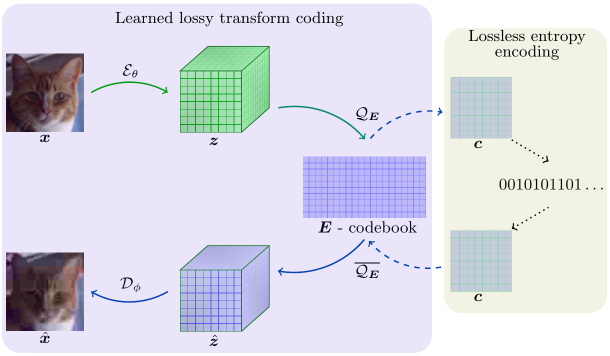
\includegraphics[width=\textwidth]{Pics/transform_coding_half.png}

\column{0.45\textwidth}

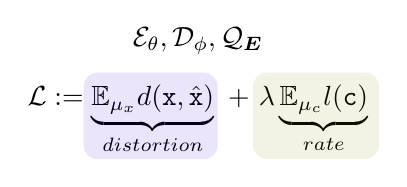
\begin{tikzpicture}
\node[inner sep=0pt] (eq) at (0, 1) {$\gEt, \gDp, \gQE$};
\node[inner sep=0pt] (eq) at (0, 0) {$
\Ls := \underbrace{\E_{\mux} d(\rvx, \hat{\rvx})}_{distortion} \ + \ \reg \underbrace{\E_{\muc} l(\rvc)}_{rate}$};

\fill[red!20!blue, fill opacity=0.1, rounded corners=5pt] (-1.45,-0.5) rectangle ++(1.7,1.1);
\fill[red!50!green, fill opacity=0.1, rounded corners=5pt] (0.7,-0.5) rectangle ++(1.6,1.1);
\end{tikzpicture}

\column{0.05\textwidth}
\
\end{columns}

\vskip 0.5cm

\onslide<2->
{%
Shannon: $l^{*}(c) = - \log p_c(c)$ $\ \Longrightarrow \ \E_{\muc} l^{*}(c) = - \E_{\muc} \log p_c(\rvc) = \Hc(\rvc)$
\[ \int_A \pc \dd \# = \sum_{\va \in \mA} \pc(\va) = \muc(\mA) \qquad \log p_c = \ ??? \quad \Hc(\rvc) = \ ???\]
\[ \alert<3->{q_c} \approx p_c \quad  - \E_{\muc} \log q_c(\rvc) \approx - \E_{\muc} \log q_c(\rvc) \quad \cHc(\rvc) \approx \Hc(\rvc)\]
}

\onslide<3->
{%
\center
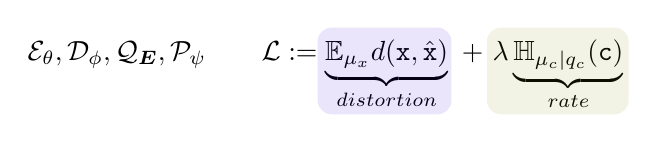
\begin{tikzpicture}
\node[inner sep=0pt] (eq) at (0, 0) {$\gEt, \gDp, \gQE, \alert{\gPp} \qquad
\Ls := \underbrace{\E_{\mux} d(\rvx, \hat{\rvx})}_{distortion} \ + \ \reg \underbrace{\alert{\cHc(\rvc)}}_{rate}$};

\fill[red!20!blue, fill opacity=0.1, rounded corners=5pt] (-0.1,-0.5) rectangle ++(1.7,1.1);
\fill[red!50!green, fill opacity=0.1, rounded corners=5pt] (2.05,-0.5) rectangle ++(1.8,1.1);
\end{tikzpicture}
}


\end{frame}



%%%%%%%%%%%%% Vector quantization %%%%%%%%%%%%%%%

\begin{frame}[t]

\structure{\Large Vector quantization}

\vskip 0.5cm

\begin{columns}[c]
\column{0.5\textwidth}
\center
Vector quantization
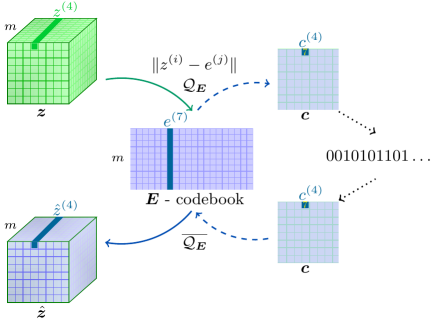
\includegraphics[width=\textwidth]{Pics/quantization_half.png}
\small message length: \alert{$d^2$}
\column{0.5\textwidth}
\center
Scalar quantization
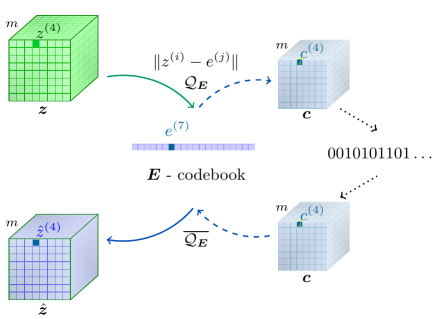
\includegraphics[width=\textwidth]{Pics/quantization_scalar_half.png}
\small message length: \alert{$d^2 m$}

\end{columns}

\vskip 0.5cm

\[\gQE: \quad \vzh^{(i)} = \argmin_{\ve^{(j)}} \Vert \vz^{(i)} - \ve^{(j)} \Vert \qquad
\evc^{(i)} = \{j : \vzh^{(i)} = \ve^{(j)} \} \]



\end{frame}


%%%%%%%%%%%%% Training problems %%%%%%%%%%%%%%%

\begin{frame}[t]

\structure{\Large Model learning - problems}

\begin{textblock*}{2.5cm}(10cm,0.2cm)
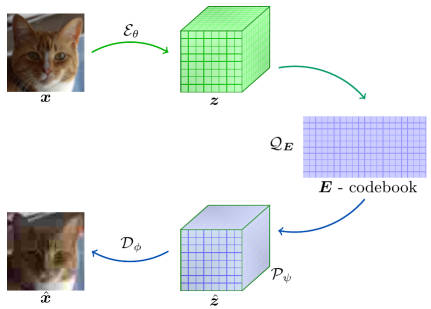
\includegraphics[width=\textwidth]{Pics/training_half.png}
\end{textblock*}

\vskip 1cm


\structure{Problem $\gQE$: quantization non-differentiable}

\vskip 0.3cm

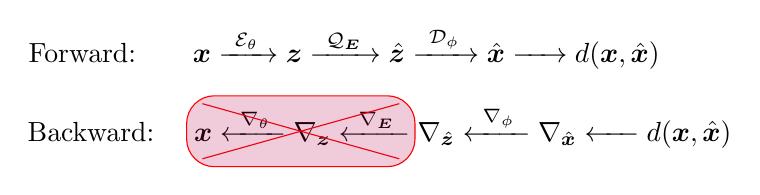
\begin{tikzpicture}

\node[inner sep=0pt] at (0, 1) {%
Forward: \, $\quad \vx \xrightarrow[]{\ \gEt \ } \vz \xrightarrow[]{\ \gQE \ } \vzh \xrightarrow[]{\ \gDp \ } \vxh \xrightarrow[]{\quad \ } d(\vx, \vxh)$%
};

\node[inner sep=0pt] at (0.45, 0) {%
Backward: $\quad \vx \xleftarrow[]{\ \nabla_{\theta} \ } \nabla_{\vz} \xleftarrow[]{\ \nabla_{\mE} \ } \nabla_{\vzh} \xleftarrow[]{\ \nabla_{\phi} \ } \nabla_{\vxh} \xleftarrow[]{\quad \ } d(\vx, \vxh)$
};

\draw[color=red] (-1.8, -0.4) to ++(2.5, 0.7);
\draw[color=red] (-1.8, 0.3) to ++(2.5, -0.7);
\fill[red!70!blue, draw=red, fill opacity=0.2, rounded corners=10pt] (-2,-0.5) rectangle ++(2.9,0.9);

% \node[color=red, inner sep=0pt] at (-0.1, -0.7) {%
% $\vzh^{(i)} = \argmin_{\ve^{(j)}} \Vert \vz^{(i)} - \ve^{(j)} \Vert$
% };
% \node[color=red, inner sep=0pt] at (-0.1, -1.2) {%
% non-differentiable
% };

\end{tikzpicture}

\vskip 0.8cm

\onslide<2->{%
\structure{Problem $\Hc$: entropy not minimized}

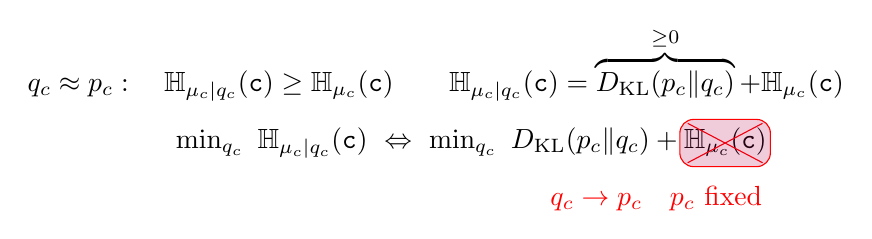
\begin{tikzpicture}

\node[inner sep=0pt] at (0, 1) {%
$q_c \approx p_c: \quad \cHc(\rvc) \geq \Hc(\rvc) \qquad \cHc(\rvc) = \overbrace{\KL(\pc \Vert \qc)}^{\geq 0} + \Hc(\rvc)$
};

\node[inner sep=0pt] at (0.45, 0) {%
$\min_{q_c} \ \cHc(\rvc) \ \Leftrightarrow \ \min_{q_c} \ \KL(\pc \Vert \qc) + \Hc(\rvc)$
};

\draw[color=red] (3.2, -0.25) to ++(0.95, 0.5);
\draw[color=red] (3.2, 0.25) to ++(0.95, -0.5);
\fill[red!70!blue, draw=red, fill opacity=0.2, rounded corners=5pt] (3.1,-0.3) rectangle ++(1.15,0.6);

\node[color=red, inner sep=0pt] at (2.8, -0.7) {%
$q_c \to p_c \quad p_c$ fixed
};
% \node[color=red, inner sep=0pt] at (3.6, -0.6) {%
% fixed
% };

\end{tikzpicture}
}


\end{frame}

%%%%%%%%%%%%% Training solutions %%%%%%%%%%%%%%%

\begin{frame}[t]

\structure{\Large Push-forward measure \& soft-quantization}

{\small
\begin{textblock*}{10cm}(1.5cm,1.2cm)
\[\mu_c[\rvc \in \mA] = \mu_c[\gTEt(\rvx) \in \mA] = \mu_x[\rvx \in \gTEt^{-1}(\mA)] \qquad \gTEt = \gQE \circ \gEt
\]
\center
\vskip -0.2cm
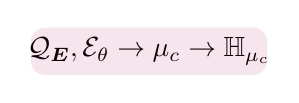
\begin{tikzpicture}
\node[inner sep=0pt] at (0, 0) {%
$\gQE, \gEt \to \muc \to \Hc$
};
\fill[red!70!blue, fill opacity=0.1, rounded corners=5pt] (-1.5,-0.3) rectangle ++(3,0.6);
\end{tikzpicture}
\end{textblock*}
\begin{textblock*}{1cm}(1cm,1.3cm)
\begin{flushleft}
\structure{1)}
\end{flushleft}
\end{textblock*}
}

\only<2->{%
\small
\begin{textblock*}{11cm}(1cm,3.2cm)
\[
\pc(c = j) =
\begin{cases}
1 & \text{if} \ \vzh = \ve^{(j)} \\
0 & \text{otherwise}
\end{cases}
\qquad h_{ce} = - \frac{1}{n} \sum_i^n \log q_c(c_i), \quad c_i \sim \muc
\]
\end{textblock*}
\begin{textblock*}{1cm}(1cm,3.2cm)
\begin{flushleft}
\structure{2)}
\end{flushleft}
\end{textblock*}

\begin{textblock*}{11cm}(1cm,4cm)
\[
\hat{p}_c(c = j) = \frac{\exp(-\sigma \Vert \vz - \ve^{(j)} \Vert)}{\sum_j^k \exp(-\sigma \Vert \vz - \ve^{(j)} \Vert)}
\qquad s_{ce} = - \frac{1}{n} \sum_{i,j}^{n,k} \hat{p}_c(c_i = j) \log \mathrm{sg}[q_c(j)]
\]
\end{textblock*}
\begin{textblock*}{1cm}(1.1cm,4.6cm)

\begin{tikzpicture}
\fill[red!70!blue, fill opacity=0.1, rounded corners=3pt] (0,0) rectangle ++(1.4,0.5);
\fill[red!70!blue, fill opacity=0.1, rounded corners=3pt] (7.6,0) rectangle ++(1.45,0.5);
\fill[red!70!blue, fill opacity=0.1, rounded corners=2pt] (9.55,0) rectangle ++(0.3,0.5);
\end{tikzpicture}
\end{textblock*}
} %onslide2

\only<3->{%
\small
\begin{textblock*}{10cm}(1.5cm,5.8cm)
\[
\vzt = \sum_j^k \hat{p}_c(c = j) \ \ve^{(j)}
\qquad \hat{d}(\vx, \vxh) = d(\vx, \gDp[\mathrm{sg}(\vzh - \vzt) + \vzt])
\]
\end{textblock*}
\begin{textblock*}{1cm}(1cm,5.8cm)
\begin{flushleft}
\structure{3)}
\end{flushleft}
\end{textblock*}
\begin{textblock*}{1cm}(3.35cm,6.1cm)

\begin{tikzpicture}
\fill[red!70!blue, fill opacity=0.1, rounded corners=3pt] (4,0) rectangle ++(1.4,0.5);
\fill[red!70!blue, fill opacity=0.1, rounded corners=3pt] (9.2,0) rectangle ++(2,0.5);
\end{tikzpicture}
\end{textblock*}
} %onslide3

\only<4->{%
\begin{textblock*}{15cm}(-1cm,7.6cm)
\[
\argmin_{\gEt, \gQE, \gDp, \gPp} \ \frac{1}{n}\sum_i^n \hat{d}(\vx_i, \vxh_i) \, + \, \alpha \, s_{ce}(\vc_i) \, + \, \beta \, h_{ce}(\vc_i), \quad \vx_i \sim \mux
\]
\end{textblock*}
\begin{textblock*}{10cm}(1.5cm,7.5cm)
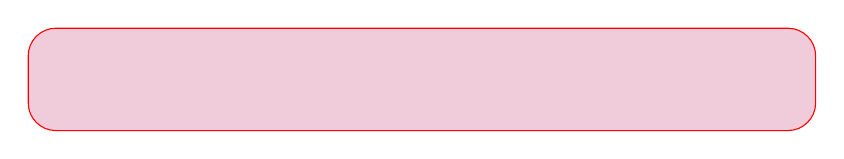
\begin{tikzpicture}
\fill[red!70!blue, draw=red, fill opacity=0.2, rounded corners=10pt] (2,1.9) rectangle ++(10,1.3);
\end{tikzpicture}
\end{textblock*}
} %onslide 4

\end{frame}

%%%%%%%%%%%%% Training solutions %%%%%%%%%%%%%%%


\begin{frame}[t]

\structure{\Large Proof of concept - experiments}

\vskip 0.5cm

\begin{tikzpicture}


\node[inner sep=0pt] at (3, 3) {%
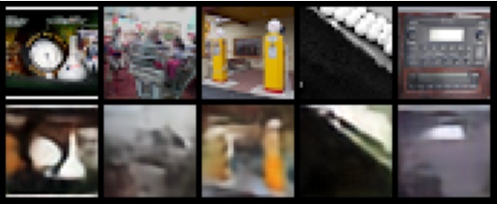
\includegraphics[width=0.3\textwidth]{Pics/reconstruct_bpp.png}
};
\node[inner sep=0pt] at (0, 0) {%
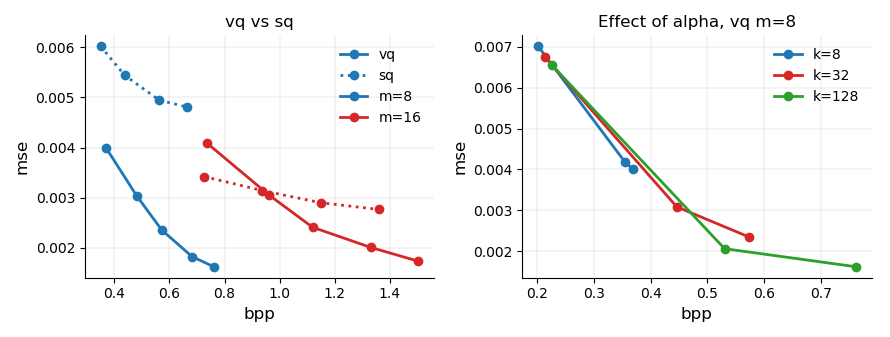
\includegraphics[width=\textwidth]{Pics/experiments.png}
};
\node[inner sep=0pt] at (3, -3) {%
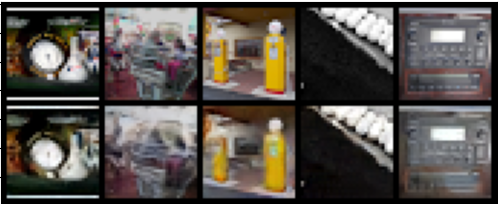
\includegraphics[width=0.3\textwidth]{Pics/reconstruct_mse.png}
};

% arrwos - lossless
\draw[color = green!50!black, thick, ->, opacity=0.5] (1.35,1.4) to ++(0.2, 0.8);
\draw[color = green!50!black, thick, ->, opacity=0.5] (4.9,-1.4) to ++(-0.7, -0.7);

\end{tikzpicture}

\begin{textblock*}{6cm}(1cm,1.1cm)
\footnotesize
\begin{flushleft}
$\gEt, \gDp$: CNN, stride-2 down-/up-sampling, 64 kernels size 3-4, 10 residual blocks with skip connections
\end{flushleft}
\end{textblock*}

\begin{textblock*}{4cm}(1cm,2cm)
\footnotesize
\[\gPp: q_c(\rvc) = \prod_i^{d^2} q_{c_i}(\rvc_i), \quad q_{c_i} = q_{c_j}\]
\end{textblock*}

\begin{textblock*}{8cm}(1cm,7.5cm)
\footnotesize
ADAM, one cycle cosine schedule\\ $\sigma=1, \ \beta=1 \qquad$
Imagenet32

\end{textblock*}



\end{frame}

% %%%%%%%%%%%%% Working diagram %%%%%%%%%%%%%%%

% \begin{frame}[t]

% \structure{\Large Transform coding with vector quantization}

% \vskip 0.5cm

% \begin{columns}
% \column{\dimexpr\paperwidth-6pt}
% \center
% \small
% \begin{tikzpicture}[scale=0.6]
% \node[inner sep=0pt] (z) at (5.5, 4.9) {$\vz$};
% \node[inner sep=0pt] (zhat) at (5.5, -1.6) {$\vzh$};
% \node[inner sep=0pt] (c) at (14.1, 4.8) {$\vc$};
% \node[inner sep=0pt] (chat) at (14.1, -0.2) {$\vc$};
% \node[inner sep=0pt] (bits) at (16.5, 3.5) {$0010101101\ldots$};
% \node[inner sep=0pt] (embed) at (10.5, 2.1) {$\mE$ - codebook};

% \node[inner sep=0pt] (quant) at (10.5, 5.8) {$\gQE$};
% \node[inner sep=0pt] (dquant) at (10.5, 0.7) {$\overline{\gQE}$};

% {\scriptsize
% \node[inner sep=0pt] (mz) at (4.5, 7.7) {$m$};
% \node[inner sep=0pt] (me) at (8, 3.4) {$m$};
% \node[inner sep=0pt] (mz) at (4.5, 1.2) {$m$};
% }


% \tikzcuboid{%
% shiftx=5.3cm,%
% shifty=6cm,%
% scale=0.50,%
% rotation=0,%
% densityx=2,%
% densityy=2,%
% densityz=2,%
% dimx=4,%
% dimy=4,%
% dimz=6,%
% front/.style={draw=green!75!black,fill=green!30!white},%
% right/.style={draw=green!50!white,fill=green!30!white},%
% top/.style={draw=green!50!white,fill=green!30!white},%
% % front/.style={draw=blue!75!black,fill=blue!25!white},%
% % right/.style={draw=blue!25!black,fill=blue!75!white},%
% % top/.style={draw=blue!50!black,fill=blue!50!white},%
% anglex=0,%
% angley=90,%
% % anglez=221.5,%
% anglez=221.5,%
% scalex=1,%
% scaley=1,%
% scalez=0.4,%
% emphedge=true,%
% emphstyle/.style={draw=black!50!green, thin},%
% shade,%
% shadeopacity=0.1,%
% }
% \tikzcuboid{%
% shiftx=5.3cm,%
% shifty=-0.5cm,%
% front/.style={draw=blue!60!white,fill=blue!70!green!20!white},%
% right/.style={draw=blue!20!white,fill=blue!70!green!20!white},%
% top/.style={draw=blue!20!white,fill=blue!70!green!20!white},%
% }

% % embeddings
% \draw[blue!25!white,xstep=0.2,ystep=0.2] (8.4,2.4) grid ++(4,2);
% \fill[blue,fill opacity=0.2] (8.4,2.4) rectangle ++(4,2);

% % c
% \draw[green!20!white,xstep=0.25,ystep=0.25] (13.2,5) grid ++(2,2);
% \fill[blue!80!green,fill opacity=0.2] (13.2,5) rectangle ++(2,2);

% % c
% \draw[green!20!white,xstep=0.25,ystep=0.25] (13.2,0) grid ++(2,2);
% \fill[blue!80!green,fill opacity=0.2] (13.2,0) rectangle ++(2,2);


% % arrows - quantizer
% \draw[color = green!60!blue, thick, ->] (7.6,6) arc[start angle = 100, end angle = 40, radius = 3];
% \draw[color = green!30!blue, thick, dashed, ->] (10.6,5) arc[start angle = 140, end angle = 80, radius = 2.5];

% % arrows - dequantizer
% \draw[color = green!30!blue, thick, ->] (10.4,1.7) arc[start angle = -40, end angle = -100, radius = 3];
% \draw[color = green!30!blue, thick, dashed, ->] (12.9,0.8) arc[start angle = -80, end angle = -140, radius = 2.5];

% % arrwos - lossless
% \draw[color = black, thick, dotted, ->] (15.2,4.95) to ++(1.2, -0.7);
% \draw[color = black, thick, dotted, <-] (15.2,2.05) to ++(1.2, 0.7);

% \fill[fill=blue!60!green, draw=blue!60!green] (14,6.8) rectangle ++(0.2,0.2);
% \node[yellow, scale=.6, inner sep=0pt] (embed) at (14.1, 6.9) {7};
% \node[blue!60!green, inner sep=0pt] (c) at (14.3, 7.3) {$c^{(4)}$};
% \fill[fill=blue!60!green, draw=blue!60!green] (14,1.8) rectangle ++(0.2,0.2);
% \node[yellow, scale=.6, inner sep=0pt] (embed) at (14.1, 1.9) {7};
% \node[blue!60!green, inner sep=0pt] (chat) at (14.3, 2.3) {$c^{(4)}$};

% %e
% \fill[fill=blue!60!green, draw=blue!60!green] (9.62,2.4) rectangle ++(0.15,2);
% \node[blue!60!green, inner sep=0pt] (z4) at (9.9, 4.7) {$e^{(7)}$};
% % z4
% \fill[blue!20!green] (5.18,6.98) rectangle ++(0.2,0.2);
% \draw[fill=blue!20!green, draw=blue!20!green] (5.2,7.2) -- (6,8) -- (6.2,8) -- (5.4,7.2) -- cycle;
% \node[blue!20!green, inner sep=0pt] (z4) at (6.3, 8.3) {$z^{(4)}$};
% % z4hat
% \fill[blue!60!green] (5.18,0.48) rectangle ++(0.2,0.2);
% \draw[fill=blue!60!green, draw=blue!60!green] (5.2,0.7) -- (6,1.5) -- (6.2,1.5) -- (5.4,0.7) -- cycle;
% \node[blue!60!green, inner sep=0pt] (z4) at (6.3, 1.8) {$\hat{z}^{(4)}$};

% \node[inner sep=0pt] (quant) at (10.5, 6.5) {$\Vert z^{(i)} - e^{(j)}\Vert$};



% \end{tikzpicture}
% \end{columns}


% \end{frame}


% %%%%%%%%%%%%% Working diagram 2 %%%%%%%%%%%%%%%

% \begin{frame}[t]

% \structure{\Large Transform coding with vector quantization}

% \vskip 0.5cm

% \begin{columns}
% \column{\dimexpr\paperwidth-6pt}
% \center
% \small
% \begin{tikzpicture}[scale=0.6]

% \node[inner sep=0pt] (z) at (5.5, 4.9) {$\vz$};
% \node[inner sep=0pt] (zhat) at (5.5, -1.6) {$\vzh$};
% \node[inner sep=0pt] (c) at (14.1, 4.75) {$\vc$};
% \node[inner sep=0pt] (chat) at (14.1, -0.6) {$\vc$};
% \node[inner sep=0pt] (bits) at (16.5, 3.5) {$0010101101\ldots$};
% \node[inner sep=0pt] (embed) at (10.5, 2.8) {$\mE$ - codebook};

% \node[inner sep=0pt] (quant) at (10.5, 5.8) {$\gQE$};
% \node[inner sep=0pt] (dquant) at (10.5, 0.7) {$\overline{\gQE}$};

% {\scriptsize
% \node[inner sep=0pt] (mz) at (4.5, 7.7) {$m$};
% \node[inner sep=0pt] (mz) at (4.5, 1.2) {$m$};
% \node[inner sep=0pt] (me) at (13.3, 7) {$m$};
% \node[inner sep=0pt] (me) at (13.3, 1.7) {$m$};
% }


% \tikzcuboid{%
% shiftx=5.3cm,%
% shifty=6cm,%
% scale=0.50,%
% rotation=0,%
% densityx=2,%
% densityy=2,%
% densityz=2,%
% dimx=4,%
% dimy=4,%
% dimz=6,%
% front/.style={draw=green!75!black,fill=green!30!white},%
% right/.style={draw=green!50!white,fill=green!30!white},%
% top/.style={draw=green!50!white,fill=green!30!white},%
% anglex=0,%
% angley=90,%
% % anglez=221.5,%
% anglez=221.5,%
% scalex=1,%
% scaley=1,%
% scalez=0.4,%
% emphedge=true,%
% emphstyle/.style={draw=black!50!green, thin},%
% shade,%
% shadeopacity=0.1,%
% }
% \tikzcuboid{%
% shiftx=5.3cm,%
% shifty=-0.5cm,%
% front/.style={draw=blue!60!white,fill=blue!70!green!20!white},%
% right/.style={draw=blue!20!white,fill=blue!70!green!20!white},%
% top/.style={draw=blue!20!white,fill=blue!70!green!20!white},%
% }

% % embeddings
% \draw[blue!25!white,xstep=0.2,ystep=0.2] (8.4,3.6) grid ++(4,0.2);
% \fill[blue,fill opacity=0.2] (8.4,3.6) rectangle ++(4,0.2);

% % c
% \tikzcuboid{%
% shiftx=13.9cm,%
% shifty=5.6cm,%
% scale=.4,
% front/.style={draw=blue!60!green!40!white,fill=blue!70!green!20!white},%
% right/.style={draw=blue!60!green!10!white,fill=blue!70!green!20!white},%
% top/.style={draw=blue!60!green!10!white,fill=blue!70!green!20!white},%
% emphedge=false,%
% }


% % c
% \tikzcuboid{%
% shiftx=13.9cm,%
% shifty=0.3cm,%
% scale=.4,
% front/.style={draw=blue!60!green!40!white,fill=blue!70!green!20!white},%
% right/.style={draw=blue!60!green!10!white,fill=blue!70!green!20!white},%
% top/.style={draw=blue!60!green!10!white,fill=blue!70!green!20!white},%
% emphedge=false,%
% }

% % arrows - quantizer
% \draw[color = green!60!blue, thick, ->] (7.6,6) arc[start angle = 100, end angle = 40, radius = 3];
% \draw[color = green!30!blue, thick, dashed, ->] (10.6,5) arc[start angle = 140, end angle = 80, radius = 2.5];

% % arrows - dequantizer
% \draw[color = green!30!blue, thick, ->] (10.4,1.7) arc[start angle = -40, end angle = -100, radius = 3];
% \draw[color = green!30!blue, thick, dashed, ->] (12.9,0.8) arc[start angle = -80, end angle = -140, radius = 2.5];

% % arrwos - lossless
% \draw[color = black, thick, dotted, ->] (15.2,4.95) to ++(1.2, -0.7);
% \draw[color = black, thick, dotted, <-] (15.2,2.05) to ++(1.2, 0.7);

% \fill[fill=blue!60!green, draw=blue!60!green] (13.8,6.4) rectangle ++(0.15,0.15);
% \node[yellow, scale=.6, inner sep=0pt] (embed) at (13.9,6.5) {7};
% \node[blue!60!green, inner sep=0pt] (c) at (14.3, 6.85) {$c^{(4)}$};
% \fill[fill=blue!60!green, draw=blue!60!green] (13.8,1.1) rectangle ++(0.15,0.15);
% \node[yellow, scale=.6, inner sep=0pt] (embed) at (13.9, 1.2) {7};
% \node[blue!60!green, inner sep=0pt] (chat) at (14.3, 1.55) {$c^{(4)}$};

% %e
% \fill[fill=blue!60!green, draw=blue!60!green] (9.62,3.6) rectangle ++(0.15,0.2);
% \node[blue!60!green, inner sep=0pt] (z4) at (9.9, 4.3) {$e^{(7)}$};
% % z4
% \fill[blue!20!green] (5.18,6.98) rectangle ++(0.2,0.2);
% \node[green!20!black, inner sep=0pt] (z4) at (5.7, 7.5) {$z^{(4)}$};
% % z4hat
% \fill[blue!60!green] (5.18,0.48) rectangle ++(0.2,0.2);
% \node[blue, inner sep=0pt] (z4) at (5.7, 1) {$\hat{z}^{(4)}$};

% \node[inner sep=0pt] (quant) at (10.5, 6.5) {$\Vert z^{(i)} - e^{(j)}\Vert$};

% \end{tikzpicture}
% \end{columns}


% \end{frame}


% % %%%%%%%%%%%%% Working Diagram 3 %%%%%%%%%%%%%%%

% \begin{frame}[t]

% \structure{\Large Transform coding with vector quantization}

% \vskip 0.5cm

% \begin{columns}
% \column{\dimexpr\paperwidth-6pt}
% \center
% \small
% \begin{tikzpicture}[scale=0.6]
% \node[inner sep=0pt] (original) at (0,6.5)
%     {
\includegraphics[width=0.12\textwidth]{Pics/cat.png}};
% \node[inner sep=0pt] (original) at (0,0)
%     {
\includegraphics[width=0.12\textwidth]{Pics/cat_hat.png}};

% \node[inner sep=0pt] (x) at (0, 5) {$\vx$};
% \node[inner sep=0pt] (xhat) at (0, -1.5) {$\vxh$};
% \node[inner sep=0pt] (z) at (5.5, 4.9) {$\vz$};
% \node[inner sep=0pt] (zhat) at (5.5, -1.6) {$\vzh$};
% \node[inner sep=0pt] (embed) at (10.5, 2.1) {$\mE$ - codebook};

% \node[inner sep=0pt] (quant) at (7.7, 3.5) {$\gQE$};
% \node[inner sep=0pt] (enc) at (2.8, 7.2) {$\gEt$};
% \node[inner sep=0pt] (dec) at (2.8, 0.2) {$\gDp$};
% \node[inner sep=0pt] (prob) at (7.7, -0.8) {$\gPp$};


% \tikzcuboid{%
% shiftx=5.3cm,%
% shifty=6cm,%
% scale=0.50,%
% rotation=0,%
% densityx=2,%
% densityy=2,%
% densityz=2,%
% dimx=4,%
% dimy=4,%
% dimz=6,%
% front/.style={draw=green!75!black,fill=green!30!white},%
% right/.style={draw=green!50!white,fill=green!30!white},%
% top/.style={draw=green!50!white,fill=green!30!white},%
% % front/.style={draw=blue!75!black,fill=blue!25!white},%
% % right/.style={draw=blue!25!black,fill=blue!75!white},%
% % top/.style={draw=blue!50!black,fill=blue!50!white},%
% anglex=0,%
% angley=90,%
% % anglez=221.5,%
% anglez=221.5,%
% scalex=1,%
% scaley=1,%
% scalez=0.4,%
% emphedge=true,%
% emphstyle/.style={draw=black!50!green, thin},%
% shade,%
% shadeopacity=0.1,%
% }
% \tikzcuboid{%
% shiftx=5.3cm,%
% shifty=-0.5cm,%
% front/.style={draw=blue!60!white,fill=blue!70!green!20!white},%
% right/.style={draw=blue!20!white,fill=blue!70!green!20!white},%
% top/.style={draw=blue!20!white,fill=blue!70!green!20!white},%
% }

% % embeddings
% \draw[blue!25!white,xstep=0.2,ystep=0.2] (8.4,2.4) grid ++(4,2);
% \fill[blue,fill opacity=0.2] (8.4,2.4) rectangle ++(4,2);



% % arrows - encoder
% \draw[color = green!70!black, thick, ->] (1.5,6.5) arc[start angle = 120, end angle = 60, radius = 2.5];

% % arrows - quantizer
% \draw[color = green!60!blue, thick, ->] (7.6,6) arc[start angle = 100, end angle = 40, radius = 3];

% % arrows - dequantizer
% \draw[color = green!30!blue, thick, ->] (10.4,1.7) arc[start angle = -40, end angle = -100, radius = 3];

% % arrows - decoder
% \draw[color = green!30!blue, thick, ->] (4,0) arc[start angle = -60, end angle = -120, radius = 2.5];






% \end{tikzpicture}
% \end{columns}


% \end{frame}


%%%%%%%%%%%% References %%%%%%%%%%%%%%%

\begin{frame}[t]

\structure{References}

\footnotesize

\vspace{0.5em}
Agustsson, E., Mentzer, F., Tschannen, M., Cavigelli, L., Timofte, R., Benini, L., \& Van Gool, L. (2017). \emph{``Soft-to-Hard Vector Quantization for End-to-End Learning Compressible Representations.''}  arXiv:1704.00648.

\vspace{0.5em}
Ballé, J., Laparra, V. \& Simoncelli, E. P. (2017). \emph{``End-to-end Optimized Image Compression.''} ICLR.

\vspace{0.5em}
Cover, T. M.  \& Thomas, T. M. (2006). \emph{``Elements of Information Theory.''} Wiley.

\vspace{0.5em}
Habibian, A., van Rozendaal, T. Tomczak, J. M., \& Cohen, T. S. (2019). \emph{``Video Compression With Rate-Distortion Autoencoders.''} ICCV.

\vspace{0.5em}
Mentzer, F., Agustsson, F., Tschannen, M., Timofte, R., Van Gool, L. (2018). \emph{``Conditional Probability Models for Deep Image Compression.''} CVPR.

\vspace{0.5em}
Sayood, K. (2012). \emph{``Introduction to Data Compression.''} Elsevier

\vspace{0.5em}
Theis, L., Shi, W., Cunningham, A. \& Huszár, F. (2017). \emph{``Lossy Image Compression with Compressive Autoencoders.''} ICLR.

\vspace{0.5em}
van den Oord, A., Vinyals, O. \& Kavukcuoglu, K. (2017). \emph{``Neural Discrete Representation Learning.''} NeurIPS.

\vspace{0.5em}
Williams, W., Ringer, S., Ash, T., Hughes, J., MacLeod, D. \& Dougherty, J. (2020). \emph{``Hierarchical Quantized Autoencoders.''} NeurIPS.

\end{frame}




\end{document}
